\subsection{Our Dynamic Frontier approach}
\label{sec:frontier}

If a batch update $\Delta^{t-} \cup \Delta^{t+}$ is small compared to the total number of edges $|E|$, then it is expected that the ranks of only a few vertices change. Our proposed \textit{Dynamic Frontier} approach incorporates this aspect, and identifies affected vertices via an incremental process.


\subsubsection{Explanation of the approach}
\label{sec:frontier-explanation}

Consider a batch update consisting of edge deletions $(u, v) \in \Delta^{t-}$ and insertions $(u, v) \in \Delta^{t+}$. We first initialize the rank of each vertex to that obtained in the previous snapshot of the graph.

\begin{figure*}[hbtp]
  \centering
  \subfigure[Initial graph]{
    \label{fig:about-frontier-01}
    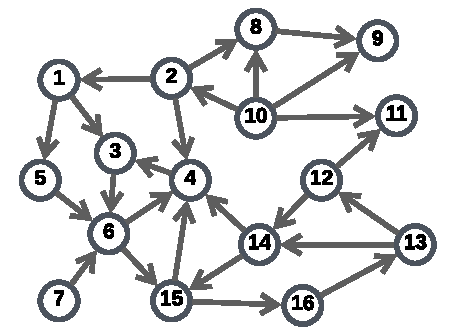
\includegraphics[width=0.23\linewidth]{out/about-frontier-01.pdf}
  }
  \subfigure[Marking affected (initial)]{
    \label{fig:about-frontier-02}
    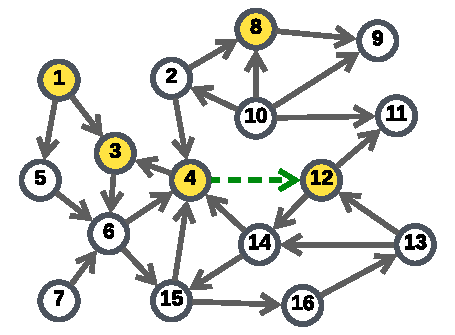
\includegraphics[width=0.23\linewidth]{out/about-frontier-02.pdf}
  }
  \subfigure[After first iteration]{
    \label{fig:about-frontier-03}
    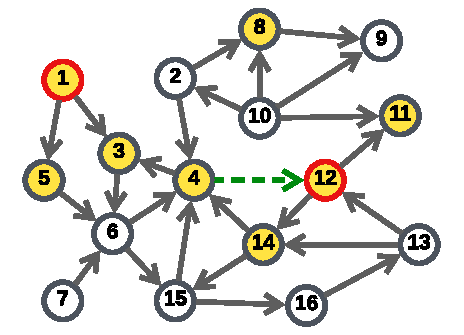
\includegraphics[width=0.23\linewidth]{out/about-frontier-03.pdf}
  }
  \subfigure[After second iteration]{
    \label{fig:about-frontier-04}
    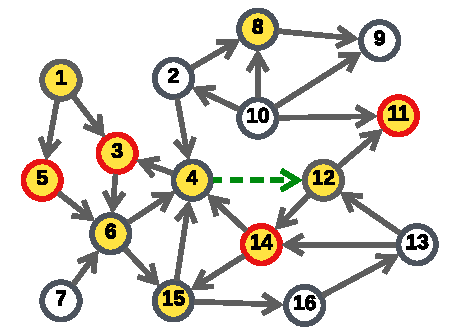
\includegraphics[width=0.23\linewidth]{out/about-frontier-04.pdf}
  } \\[-2ex]
  % \subfigure[]{
  %   \label{fig:about-frontier-05}
  %   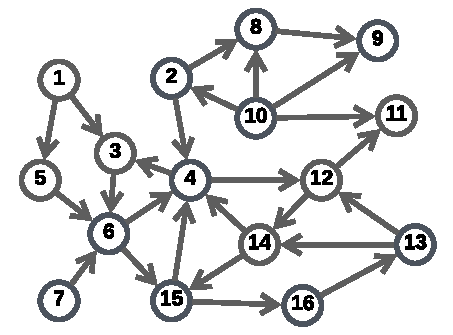
\includegraphics[width=0.18\linewidth]{out/about-frontier-05.pdf}
  % }
  \caption{Illustration of the \textit{Dynamic Frontier} approach through a specific example. The initial graph consists of $16$ vertices and $25$ edges. The graph is then updated with an edge insertion $(4, 12)$, and an edge deletion $(2, 1)$. Accordingly, the outgoing neighbors of vertices $4$ ($3$ and $12$) and $2$ ($1$, $4$, and $8$) are marked as affected (shown with yellow fill). When the ranks of these affected vertices are computed in the first iteration, it is found that change in rank of vertices $1$ and $12$ exceeds the frontier tolerance $\tau_f$ (shown with red border). Thus, outgoing neighbors of vertices $1$ ($3$ and $5$) and $12$ ($11$ and $14$) are also marked as affected. In the second iteration, the change in rank of vertices $3$, $5$, $11$, and $14$ is greater than $\tau_f$ --- thus their outgoing vertices are marked as affected. In the subsequent iteration, the ranks of affected vertices are again updated. If the change in rank of every vertex is within iteration tolerance $\tau$, the ranks of vertices have converged, and the algorithm terminates.}
  \label{fig:about-frontier}
\end{figure*}


\paragraph{Initial marking of affected vertex on edge deletion/insertion:}

For each edge deletion/insertion $(u, v)$, we initially mark the outgoing neighbors of the vertex $u$ in the previous $G^{t-1}$ and current graph snapshot $G^t$ as affected.

\paragraph{Incremental marking of affected vertices upon change in rank of a given vertex:}

Next, while performing PageRank computation, if the rank of any affected vertex $v$ changes in an iteration by an amount greater than the \textit{frontier tolerance} $\tau_f$, we mark its outgoing neighbors as affected. This process of marking vertices continues in every iteration.


\subsubsection{A simple example}

Figure \ref{fig:about-frontier} shows an example of the \textit{Dynamic Frontier} approach. The initial graph, shown in Figure \ref{fig:about-frontier-01}, comprises $16$ vertices and $25$ edges. Subsequently, Figure \ref{fig:about-frontier-02} shows a batch update applied to the original graph involving the deletion of an edge from vertex $2$ to $1$ and the insertion of an edge from vertex $4$ to $12$. Following the batch update, we perform the initial step of the \textit{Dynamic Frontier} approach, marking outgoing neighbors of $2$ and $4$ as affected, i.e., $1$, $3$, $4$, $8$, and $12$ are marked as affected (indicated with a yellow fill). Note that vertex $2$ is not affected as it is a source of the change while vertex $4$ being a neighbour of $2$ is marked as affected. Now, we are ready to execute the first iteration of PageRank algorithm.

During the first iteration (see Figure \ref{fig:about-frontier-03}), the ranks of affected vertices are updated. It is observed that the rank changes of vertices $1$ and $12$ surpass the frontier tolerance $\tau_f$ (highlighted with a red border). In response to this, we incrementally mark the outgoing neighbors of $1$ and $12$ as affected, i.e., vertices $5$, $11$, and $14$. 

During the second iteration (see Figure \ref{fig:about-frontier-04}), the ranks of affected vertices are again updated. Here, its is observed that the change in rank of vertices $3$, $5$, $11$, and $14$ is greater than frontier tolerance $\tau_f$. Thus, we mark the outgoing neighbors of $3$, $5$, $11$, and $14$ as affected, namely vertices $4$, $6$, and $15$.

In the subsequent iteration, the ranks of affected vertices are again updated. If the change in rank of each vertex is within iteration tolerance $\tau$, the ranks of vertices have converged, and the algorithm terminates.




\subsection{Synchronous vs Asynchronous implementation}

In a synchronous implementation, separate input and output rank vectors are used, ensuring deterministic results for parallel algorithms through vector swapping at the end of each iteration. In contrast, an asynchronous implementation utilizes a single rank vector, potentially achieving faster convergence and eliminating memory copies for unaffected vertices in dynamic approaches\ignore{, but introduces non-deterministic results in parallel algorithms}.

To check whether a synchronous or an asynchronous implementation is suitable for \textit{Dynamic Frontier} PageRank, we attempt both the implementations for \textit{Static}, \textit{Naive-dynamic}, \textit{Dynamic Traversal}, and \textit{Dynamic Frontier} PageRank on batch updates (consisting purely of edge insertions) of size $10^{-7}|E|$ to $0.1|E|$. Figure \ref{fig:measure-affected} shows the average relative runtime with asynchronous implementations of each approach compared to their respective synchronous implementations. Results indicate that asynchronous implementations, especially for smaller batch sizes.\ignore{This is due to a somewhat faster convergence and the absence of copy overhead (for \textit{Dynamic Traversal} and \textit{Dynamic Frontier} approaches).} Accordingly, we use the asynchronous implementations of \textit{Naive-dynamic}, \textit{Dynamic Traversal}, and \textit{Dynamic Frontier} PageRank.




\subsection{Determination of Frontier tolerance ($\tau_f$)}

We now measure a suitable value for frontier tolerance $\tau_f$ that allows us to minimize the number of vertices we process (after marking them as affected), while ensuring that we obtain ranks with the desired tolerance, i.e. we obtain ranks with no higher error than \textit{Static} PageRank for the same tolerance setting. For this, we adjust frontier tolerance $\tau_f$ from $\tau$ to $\tau / 10^5$ and obtain ranks of vertices with the \textit{Dynamic Frontier} approach on batch updates (consisting purely of edge insertions) of size $10^{-7}|E|$ to $0.1|E|$.

Figure \ref{fig:adjust-frontier} illustrates the average relative runtime and rank error (in comparison to ranks obtained with reference Static PageRank) using the \textit{Dynamic Frontier} approach. The figure suggests that as $\tau_f$ increases, runtime decreases, but it is accompanied by an increase in error. A frontier tolerance $\tau_f$ set at $\tau/10^4$ or $\tau/10^5$ yields ranks with lower error than \textit{Static} PageRank, making them acceptable for uniformly random batch updates. To err on the side of caution, we opt for a frontier tolerance of $\tau_f = \tau/10^5$.

\begin{figure*}[!hbt]
  \centering
  \subfigure{
    \label{fig:approach-async--mean}
    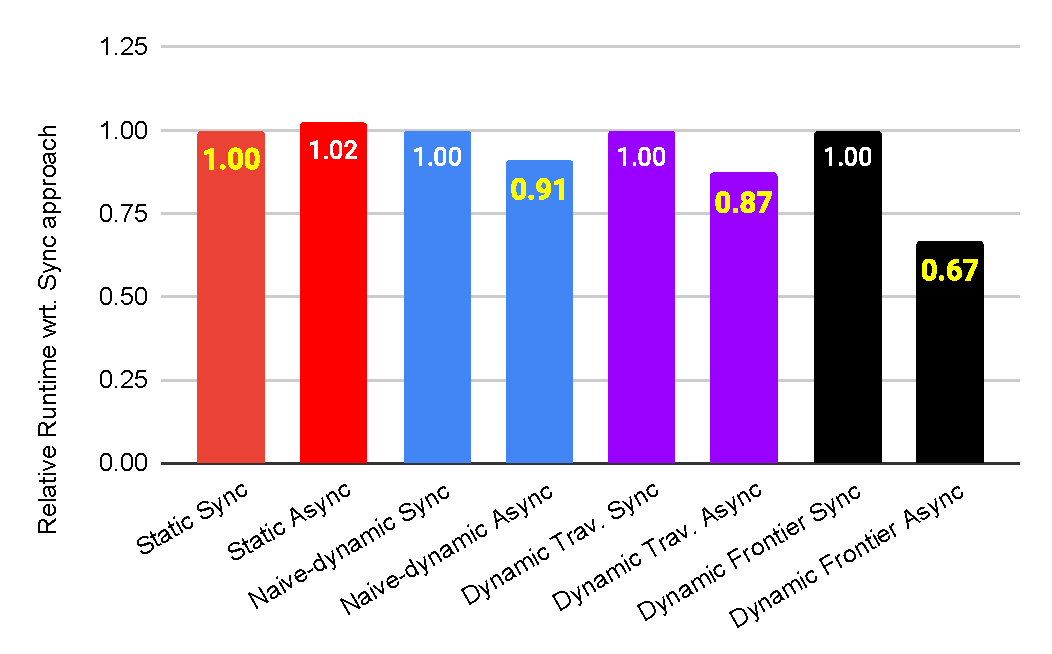
\includegraphics[width=0.48\linewidth]{out/approach-async-mean.pdf}
  }
  \subfigure{
    \label{fig:approach-async--batch}
    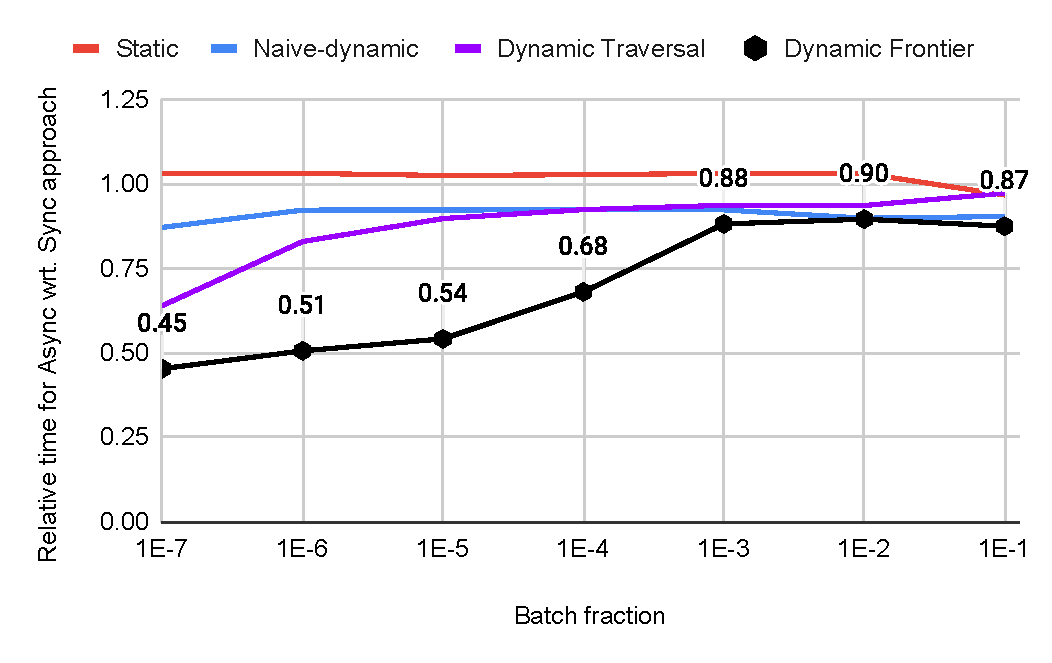
\includegraphics[width=0.48\linewidth]{out/approach-async-batch.pdf}
  } \\[-2ex]
  \caption{Average Relative runtime with asynchronous implementations of \textit{Static}, \textit{Naive-dynamic}, \textit{Dynamic Traversal}, and \textit{Dynamic Frontier} approach compared to their respective synchronous implementations, on batch updates of size $10^{-7}|E|$ to $0.1|E|$ (right), and overall (left). The results indicate that asynchronous implementations are faster than synchronous ones, especially for smaller batch sizes. This is due to a somewhat faster convergence and the absence of copy overhead (for \textit{Dynamic Traversal} and \textit{Dynamic Frontier} approaches).}
  \label{fig:approach-async}
\end{figure*}

\begin{figure}[!hbt]
  \centering
  \subfigure{
    \label{fig:adjust-frontier--runtime}
    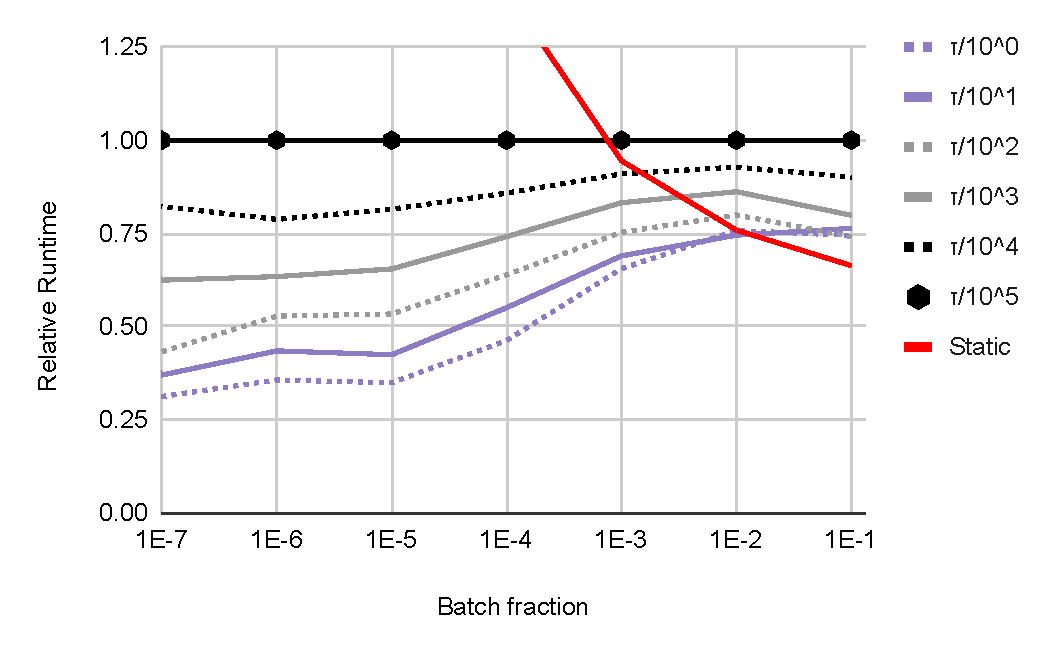
\includegraphics[width=0.98\linewidth]{out/adjust-frontier-runtime.pdf}
  } \\[-1ex]
  \subfigure{
    \label{fig:adjust-frontier--error}
    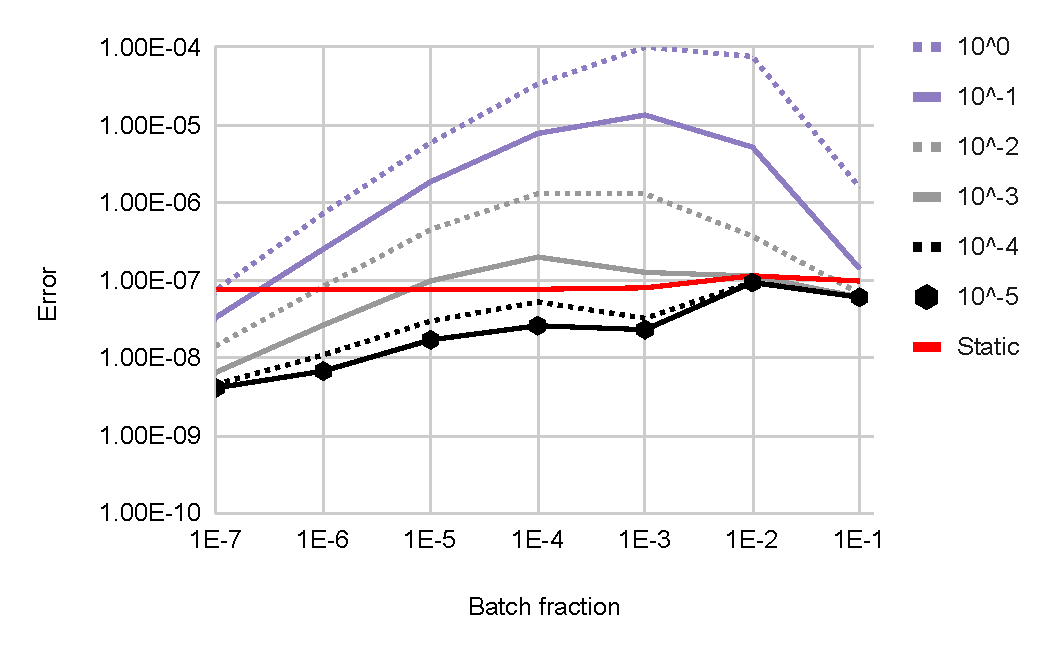
\includegraphics[width=0.98\linewidth]{out/adjust-frontier-error.pdf}
  } \\[-2ex]
\caption{Adjust Frontier. The error is averaged over the graphs in Table \ref{tab:dataset}.}
  \label{fig:adjust-frontier}
\end{figure}

\begin{algorithm}[!hbt]
\caption{Our parallel Dynamic Frontier PageRank.}
\label{alg:frontier}
\begin{algorithmic}[1]
\Require{$G^{t-1}, G^t$: Previous, current input graph}
\Require{$\Delta^{t-}, \Delta^{t+}$: Edge deletions and insertions (input)}
\Require{$R^{t-1}$: Previous rank vector}
\Ensure{$R$: Current rank vector}
\Ensure{$\Delta r$: Change in rank of a vertex}
\Ensure{$\Delta R$: $L\infty$-norm between previous and current ranks}
\Ensure{$\tau, \tau_f$: Iteration, frontier tolerance}
\Ensure{$\alpha$: Damping factor}

\Statex

\Function{dynamicFrontier}{$G^{t-1}, G^t, \Delta^{t-}, \Delta^{t+}, R^{t-1}$}
  \State $R \gets R^{t-1}$
  \State $\rhd$ Mark initial affected
  \ForAll{$(u, v) \in \Delta^{t-} \cup \Delta^{t+} \textbf{in parallel}$} \label{alg:frontier--mark-begin}
    \ForAll{$v' \in (G^{t-1} \cup G^t).out(u)$}
    \State Mark $v'$ as affected
    \EndFor
  \EndFor \label{alg:frontier--mark-end}
  \ForAll{$i \in [0 .. MAX\_ITERATIONS)$} \label{alg:frontier--compute-begin}
    \State $\Delta R \gets 0$
    \ForAll{affected $v \in V^t$ \textbf{in parallel}}
      \State $r \gets (1 - \alpha)/|V^t|$
      \ForAll{$u \in G^t.in(v)$}
        \State $r \gets r + \alpha * R[u] / |G^t.out(u)|$
      \EndFor
      \State $\Delta r \gets |r - R[v]|$ \textbf{;} $R[v] \gets r$
      \State $\Delta R \gets max(\Delta R, \Delta r)$
      \State $\rhd$ Is rank change $>$ frontier tolerance?
      \If{$\Delta r > \tau_f$} \label{alg:frontier--remark-begin}
        \ForAll{$v' \in G^t.out(v)$}
          \State Mark $v'$ as affected
        \EndFor
      \EndIf \label{alg:frontier--remark-end}
    \EndFor
    \State $\rhd$ Ranks converged?
    \If{$\Delta R \le \tau$} \textbf{break}
    \EndIf
  \EndFor \label{alg:frontier--compute-end}
  \State \ReturnInline{$R$} \label{alg:frontier--return}
\EndFunction
\end{algorithmic}
\end{algorithm}




%% Requires (parameters):
% G(V, E): a directed unweighted graph
% R: initial ranks (1/N for static)

%% Parameter values:
% MAX\_ITERATIONS = 500
% DAMPING\_FACTOR = 0.85
% TOLERANCE = 10^-10





\subsection{Our Dynamic Frontier PageRank implementation}

Algorithm \ref{alg:frontier} shows our implementation of \textit{Dynamic Frontier} PageRank, which is designed to compute the PageRank of vertices in a graph while efficiently handling dynamic changes in the graph structure over time. The algorithm takes as input the previous and current versions of the graph, edge deletions and insertions in the batch update, and the previous rank vector.

It begins by marking the initially affected vertices based on the edge deletions $\Delta^{t+}$ and insertions $\Delta^{t-}$ in parallel (lines \ref{alg:frontier--mark-begin}-\ref{alg:frontier--mark-end}). It then enters an iterative computation phase (lines \ref{alg:frontier--compute-begin}-\ref{alg:frontier--compute-end}), where it updates the rank of each affected vertex. The PageRank computation is performed in parallel for each affected vertex $v$, considering the incoming edges $G^t.in(v)$. The algorithm checks whether the change in rank $\Delta r$ exceeds the frontier tolerance $\tau_f$, and marks its out-neighbor vertices as affected if so. The iteration continues until either the net change in ranks $\Delta R$ (which is equal to the $L\infty$-norm between the previous and the current ranks) falls below the iteration tolerance $\tau$, or a maximum number of iterations is reached $MAX\_ITERATIONS$. In line \ref{alg:frontier--return}, the final rank vector $R$ is returned.




% Dynamic Frontier (DF) approach
% Adjusting tolerance, Frontier tolerance, Mark DelRank / DelContrib
% Dynamic Frontier optimizations
% Edge-balanced approach (Chunk size)
